\header{
    \section{Sont les filles de la Rochelle} \label{sont-les-filles-de-la-rochelle}
    %
    %
    
    \insertComment{Inspirée du siège de la Rochelle de 1628, écrite dans la foulée.}{}
}

\enluminure{4}{\href{https://www.youtube.com/watch?v=4YFw5383ovU}{S}}{ont} les filles de La Rochelle
\\Qu'ont armé un bâtiment ~~\bissimple
\\Elles ont la cuisse légère
\\Et la fesse à l'avenant
\\\\\textbf{Refrain :}
\\Ah' la feuille s'envole, s'envole
\\Ah! la feuille s'envole au vent
\\\\Sont parties aux Amériques
\\Un matin, la voile au vent~~ \bissimple
\\Ont choisi pour capitaine
\\Une fille de vingt ans.
\\\\Nous n'avons pas besoin d'hommes,
\\Disaient-elles à l'avenant ~~~~~~~~~~~~\bissimple
\\Mais au bout de six semaines
\\Elles avaient le cul brûlant.
\\\\Un beau soir, une frégate
\\Apparut sur l'Océan,~~~~~~ \bissimple
\\Pleine de jolis pirates,
\\De beaux gars appétissants
\\\\Elles allèrent à l'abordage
\\A coups d'sabre et à coups d'dents~ \bissimple
\\Elles y prirent l'avantage
\\Et se ram'nèrent des galants.
\\\\Et sous la lune jolie,
\\Etendues sans vêtements,~~~~~ \bissimple
\\Elles ont écarté les cuisses
\\Toutes sur le gaillard d'avant.
\breakpage
Ont baisé à perdre haleine
\\Jusqu'au clair soleil levant ~\bissimple
\\Et c'était la capitaine
\\Qui menait le mouvement.
\\\\Le lend'main le beau navire
\\Repartit vers le couchant ~~~~~~\bissimple
\\Et les filles de La Rochelle
\\Le cul frais allaient chantant:
\\\\"J'ai perdu mon pucelage
\\Au milieu de l'Océan~~~~~~~ \bissimple
\\ll est parti vent arrière
\\Reviendra z'en louvoyant".
\\
\bigskip
\begin{center}
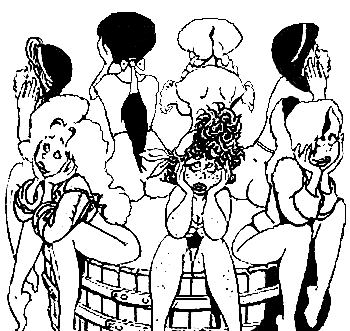
\includegraphics[width=1\textwidth]{images/rochelle.png}
\end{center}

\breakpage